% Subsection on jack

Le premier élément nécessaire pour ce hands-on est un \emph{connecteur jack femelle}, tel celui de la Figure \ref{fig:jack_pic}. Ce connecteur permet d'amener les signaux audio sur la breadboard, en y connectant une source audio (smartphone, ordinateur ou autre) via un câble jack mâle-mâle. Malheureusement, les connecteurs jacks ne peuvent pas être insérés tels quels dans les breadboards. Cela peut être réolu simplement via la soudure de quelques fils.\\

\begin{minipage}[c]{\textwidth}
	\centering
	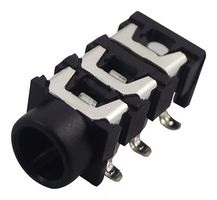
\includegraphics[width=0.3\textwidth]{figures/jack.jpg}
	\captionof{figure}{Photo du connecteur jack femelle.}
	\label{fig:jack_pic}
\end{minipage}
\vspace{1cm}